\pdfobjcompresslevel=0
\pdfcompresslevel=9
\pdfminorversion=7
\documentclass[letterpaper, 12, one column]{article}
%% packages %%

% === Rasterizar PDFs pesados automáticamente ===
\usepackage{graphicx,xifthen}
\newif\iffigdraft
% \figdrafttrue   % ← descomenta para compilar rápido (raster a 150 dpi)
% \figdraftfalse  % ← descomenta para calidad final (raster a 300 dpi)




\usepackage{tikz}
\usepackage{amsmath}

\usetikzlibrary{angles, quotes}

\usepackage{hyperref}
\usepackage{graphics,color}
\usepackage[table]{xcolor} 
\usepackage{tabularray}
\usepackage{epsfig} 
\usepackage{psfrag,epsfig}
\usepackage{graphics}                       % Soporte gráfico
\usepackage{changepage}
\usepackage{graphicx}   
\usetikzlibrary{arrows.meta}% Soport\e gráfico adicional
\usepackage{epstopdf}
\usepackage{float}
\usepackage{mathptmx} 
\usepackage{times} 
\usepackage{amsmath}
\usepackage{amssymb}  
\usepackage{bm}  
\usepackage{rotating} % <-- Asegúrate de incluir esto en el preámbulo
\usetikzlibrary{angles, quotes,shapes}
\usepackage{color}
\usepackage{multirow} 
\usepackage{cleveref}
\usepackage{cite}
\usepackage{arydshln}
\usepackage{booktabs}
\usepackage{microtype}
\usepackage{longtable}
\usepackage{lscape}
\usepackage{multirow}
\usepackage{array}
\usepackage{xcolor}
\usepackage{subcaption}
%\usepackage[caption=false]{subfig}
\usepackage{tikz}
    \usetikzlibrary{positioning,mindmap,arrows.meta,bending}
    \usetikzlibrary{mindmap, backgrounds, calc} % Mindmap drawing library 
    \usetikzlibrary{positioning,shapes,shadows,arrows, shapes.geometric}
\usepackage{adjustbox}
\newcommand{\gc}[1]{\textcolor[rgb]{1.00,0.00,0.00}{#1}}
\providecommand{\var}[1]{{\ensuremath{var}}\{#1\}}
\DeclareMathOperator{\tire}{\negthinspace-\negthinspace}
\DeclareRobustCommand{\legend}[1]{%
	\textcolor{#1}{\rule{1ex}{2ex}}%
}
\newcommand{\lineplot}[1]{
	\textcolor{#1}{\rule{1.5ex}{0.3ex}}%
}

%\setbeamertemplate{itemize/enumerate body begin}{\large}
%\usepackage{enumitem}
\newcommand{\tikzmark}[1]{\tikz[baseline,remember picture] \coordinate (#1) {};}

\usepackage{booktabs,colortbl,pifont}
\definecolor{completed}{RGB}{220,235,220}   % light green
\definecolor{writing}{RGB}{255,235,200}     % light orange
\newcommand{\cmark}{\ding{52}}   % ✔
\newcommand{\wmark}{\ding{118}}  % ⌘ (for “writing” phase) – choose any
\renewcommand{\arraystretch}{1.15}
%% commands %%
\DeclareMathAlphabet{\mathantt}{OT1}{antt}{li}{it}
\DeclareMathAlphabet{\mathpzc}{OT1}{pzc}{m}{it}
\providecommand{\abs}[1]{\lvert#1\rvert}
\providecommand{\norm}[1]{\lVert#1\rVert} 
\providecommand{\ppunto}[2]{\langle#1,#2\rangle}
\providecommand{\dist}[2]{{ d}(#1, #2)} 
\providecommand{\promed}[1]{{\fam=8 E}\{#1\}}
\providecommand{\cov}[2]{{\fam=7 cov}\{#1, #2\}}
\providecommand{\gaus}[2]{{\fam=6 N}(#1 #2)}
\providecommand{\unif}[1]{{\fam=6 U}(#1 )} 
\providecommand{\ve}[1]{{\bm {#1}}} 
\providecommand{\mat}[1]{{\bm {#1}}} 
\providecommand{\est}[1]{{\widetilde {#1}}}
\providecommand{\diag}[1]{{\rm{diag}}(#1)}
\newcommand{\jc}[1]{\textcolor[rgb]{0.00,0.0,1.00}{#1}}


\usepackage{longtable}
\usepackage{lscape}
\usepackage{multirow}
\usepackage{array}
\usepackage{xcolor}
\usepackage{xcolor}
\usepackage{soul}
\usetikzlibrary{positioning, arrows.meta}
%\usepackage{subcaption}

%\usepackage[hyperindex, colorlinks, citecolor=blue, linkcolor=blue, breaklinks=true, bookmarksopen]{hyperref}
\newcommand{\fou}{\ensuremath{\mathcal{F}}}%Para crear la F de Fourier
\newcommand{\ent}{\ensuremath{\mathbb{Z}}}%Pa crear algo parecido a la Z de enteros
\newcommand{\Z}{\ensuremath{\mathbb{Z}}}%Pa crear algo parecido a la R de reales
\newenvironment{definición}{\it \vspace{.4cm}\hrule \vspace{.2cm}}{\par\sf \vspace{.2cm}\rm\hrule\vspace{.4cm}}

%%%%%%%%%%%%%%%%%%%%%%%%%%%%%%% Custom Commands %%%%%%%%%%%%%%%%%%%%%%%%%%%%%%%%
\usepackage{tikz}
\usetikzlibrary{external}
\providecommand{\abs}[1]{\left| #1 \right|}
\providecommand{\norm}[1]{{\lVert #1 \rVert}_2}
\providecommand{\normH}[1]{{\lVert #1 \rVert}_\mathscr{H}}
\providecommand{\promedd}[2]{\mathbb{E}_{#1}\!\left\{#2\right\}}% op{\tiny }erador de promedio
\providecommand{\prodpunto}[2]{\left\langle #1,#2\right\rangle}

\providecommand{\paren}[1]{\!\left(\!#1\!\right)\!}
\newcommand{\T}{\top\!}
\newcommand{\p}{\prime\!}

\providecommand{\median}[1]{\text{median}\!\left(\!#1\!\right)}
\providecommand{\sign}[1]{\text{sign}\!\left(\!#1\!\right)}
\providecommand{\ve}[1]{{\bm{#1}}} %
\providecommand{\tr}[1]{{\operatorname{tr}\left({#1}\right)}}
\providecommand{\mat}[1]{{\bm{#1}}} %
\providecommand{\var}[1]{{\operatorname{var}}\left\{#1\right\}}
\providecommand{\map}[1]{\varphi\!\left(#1\right)}
\newcommand{\Real}{\mathbb{R}}
\newcommand{\N}{\mathbb{N}}
%\newcommand{\Z}{\mathbb{Z}}
\newcommand{\unos}{\ve{1}}
\providecommand{\kernel}[2]{\kappa\negthinspace\left(#1,\negthinspace#2\right)}
\DeclareMathOperator{\subconj}{\negthinspace\subset\negthinspace }
\DeclareMathOperator{\en}{\!\in\!}
\DeclareMathOperator{\igual}{\negthinspace=\negthinspace} 
\DeclareMathOperator{\diferente}{\negthinspace \neq \negthinspace}
% \DeclareMathOperator{\dist}{\operatorname{d}}

%\DeclareMathOperator{\xx}{\negthickspace\times\negthickspace}
\providecommand{\s}[1]{\negthinspace#1\negthinspace}%

\usepackage[normalem]{ulem}
%% Color text %%
\providecommand{\falta}[1]{\textcolor{green}{\underline{#1}}}
\providecommand{\duda}[1]{\textcolor{yellow}{{#1}}}
\providecommand{\am}[1]{\textcolor{green}{#1}}
\providecommand{\je}[1]{\textcolor{blue}{#1}}

% Note: pifont, \cmark and \xmark already defined at line 73-77
\definecolor{mypink1}{rgb}{0.858, 0.188, 0.478}
\usepackage{graphicx,xifthen,xstring} % <— necesario

\newif\iffigdraft
% \figdrafttrue   % ← modo rápido (150 dpi)
\figdraftfalse    % ← modo final (300 dpi)

\newcommand{\rasterpdffile}[3][]{%
  % Uso: \rasterpdffile[<dpi>]{ruta/figura.pdf}{<ancho>}
  \def\dpi{#1}%
  \ifthenelse{\isempty{#1}}{\iffigdraft\def\dpi{150}\else\def\dpi{300}\fi}{}%
  \StrBefore{#2}{.pdf}[\base]%
  \IfFileExists{\base.ras@\dpi.png}{}{%
    \immediate\write18{gs -q -dSAFER -dBATCH -dNOPAUSE -sDEVICE=pngalpha -r\dpi
      -dFirstPage=1 -dLastPage=1 -o "\base.ras@\dpi.png" "#2"}%
  }%
  \includegraphics[width=#3]{\base.ras@\dpi.png}%
}

 % {A multimodal deep learning approach with preserved interpretability to support remote sensing tasks}}

\title{Explainable Deep Learning Framework for Estimating and Generating Magnetic Domains from Hamiltonian Parameterss}
\author{\emph{PhD Thesis Proposal}\\ Juan Sebastián Méndez Rondón \\ \texttt{\small jumendezro@unal.edu.co} \\ \\ \\ 
Advisor: Prof. Andr\'es Marino \'Alvarez-Meza \\ \small{Universidad Nacional de Colombia - Sede Manizales} \\ \small{Facultad de Ingenier\'ia y Arquitectura} \\ \texttt{\scriptsize   amalvarezme@unal.edu.co} 
\\ \\ 
Co-Advisor: Prof. Jorge Ivan Montes\\ \small{Universidad Nacional de Colombia - Sede la paz}  \\ \texttt{\scriptsize  jimontesm@unal.edu.co } }

%Lack of interpretability
\date{Doctorado en Ingenier\'ia - Autom\'atica \\ Universidad Nacional de Colombia - Sede Manizales}
% ====== PREÁMBULO COMPATIBLE CON TUS TABLAS ======
\usepackage{booktabs,tabularx,array,changepage,float}
\usepackage{soul,xcolor}
\sethlcolor{yellow!20}

% Macros de ancho usadas por tus tablas
\newlength{\fulllength}  \setlength{\fulllength}{\textwidth}
\newlength{\extralength} \setlength{\extralength}{0pt}

% Columna centrada expandible "C" para tabularx
\newcolumntype{C}{>{\centering\arraybackslash}X}


\begin{document}
\maketitle
\section{Abstract}
The study of magnetic domain structures in nanoscale materials is essential for advancing
emerging technologies in spintronics, biomedicine, and energy storage \cite{Wang2022, Rarokar2024, Lak2021}. 
Magnetic nanoparticles and nanodots exhibit complex spin textures—such as vortices, skyrmions,
and stripe domains—that determine their functional behavior in applications ranging from magnetic
memory bits to targeted hyperthermia \cite{Wang2022, Lak2021, Zelent2021}. Understanding and controlling
these states requires a deep connection between the parameters of the magnetic Hamiltonian
(exchange, anisotropy, Dzyaloshinskii–Moriya interaction, external field, and temperature) and the
resulting spatial spin configurations \cite{Zelent2021, Ga2022, Fert2023}.

However, several fundamental challenges persist at the nanoscale. The first is the nonlinearity and
high dimensionality of the mapping between physical parameters and domain patterns, which prevents
direct analytical inversion \cite{WangMicromag2024, DeepMLHam2024}. The second is degeneracy:
distinct combinations of Hamiltonian parameters can yield visually similar configurations, complicating
inverse identification \cite{Feng2024, Liu2023}. Third, experimental limitations—such as noise, finite
probe resolution, tip–sample convolution in MFM, and sample variability—hinder quantitative
interpretation of MFM or SP-STM images \cite{Makarova2022, Bagchi2024}. Finally, the computational cost
of atomistic or micromagnetic simulations restricts large-scale parameter sweeps, limiting predictive
exploration of material regimes \cite{WangMicromag2024, MuMax3docs}.

Deep learning has emerged as a powerful tool to bridge this gap. The inverse problem—inferring
physical parameters from magnetic domain images—has been successfully addressed using CNNs and
explainable regression frameworks \cite{Kong2023, AIP2022, DeepMLHam2024}. The direct problem—
generating domain configurations from parameters—has been explored in materials science using
generative models such as VAEs and conditional GANs \cite{MicroVAE2023, Ronne2024}. These methods
can reproduce general morphologies but suffer from poor interpretability, instability under noise, limited
generalization, and lack of physical constraints \cite{Feng2024, Park2024, MicroVAE2023}.


% AGREGAR EL PARRAFO INTRODUCTORIO ASOCIADO A LAS TAREAS QUE SE VAN A GENERAR. -- > REVISAR CON ANDRES MARINO.

%% FIGURA DEL PROBLEMA INVERSO Y DIRECTO --CHECK

%% CAMBIAR EL PROBLEMA MIXTO DEGENERAY OF CONFIGURATIONS --CHECK
%% 2 parrafos uno que conceptualmente explique que es  y las posibles causas segun la fisica. --CHECK
%% LOW QUALITY DATA. 

%% explicabilidad fisica.
%% RESUMIR EN UNA TABLA O DIBUJO EL ESTADO DEL ARTE.
%% tabla con items para los proyectos futuros.




% TUTORIAL DE REDES INFORMADAS POR LA FISICA -- MIRAR COMO LLEVARLO A UN METODOLOGIA DE OPTIMAZCIÓN BAYESIANA. - QUE SEA EXPLICABLE. COMO PUEDO SINTONIZAR DICHOS CON INTERPRETABILIDAD.
%% CON UN EJERCICIO BASICO.


Recently, diffusion-based models have achieved state-of-the-art performance in conditional image
synthesis and inverse design across materials science \cite{Alverson2024, Chen2024, SyMat2023}. Yet,
their application to magnetic systems remains underexplored, and existing generative strategies rarely
enforce physical consistency—such as energy minimization or Hamiltonian symmetry—limiting their use
for predictive materials discovery \cite{Ronne2024, Park2024}.


This work proposes a unified deep learning framework for direct and inverse estimation of magnetic
Hamiltonian parameters and textures. The approach integrates physics-informed generative architectures—
such as conditional diffusion models guided by Hamiltonian-based embeddings or energy priors—
with interpretable regression models in a cycle-consistent physical loop that enforces coherence in
both directions. Bayesian hyperparameter optimization will be used to explore architectures efficiently
and enhance robustness \cite{Sparks2024, Optuna2022}.


\section{Motivation}

%1.1. Contexto general: el magnetismo a nanoescala

The study of magnetic systems at the nanoscale has gained strategic importance in
modern materials science \cite{Wang2022, Lak2021}. In particular, magnetic nanoparticles (MNPs) and nanodots
constitute platforms where spin interactions and collective quantum properties give
rise to emergent phenomena of great scientific and technological interest \cite{Jiang2023, Rarokar2024}. At these
scales, the balance between exchange interactions, anisotropy, Dzyaloshinskii–Moriya
interaction (DMI), and external magnetic fields generates a wide variety of magnetic
textures—vortices, skyrmions, helical domains, and labyrinthine configurations \cite{Ga2022, Fert2023, Tokura2021}. These
structures determine the magnetic response, thermal stability, and switching dynamics
of the material, which are key aspects for functionality in advanced devices \cite{Song2023, Wang2022}.


\begin{figure}[H]
    \centering
    \includegraphics[width=0.75\textwidth]{Figures/magneticTexture.jpg}
    \caption{ Magnetic domains configurations }
    \label{fig:skyrmions_textures}
\end{figure}

%1.2. Relevancia aplicada: por qué las nanopartículas magnéticas importan

Magnetic nanoparticles and nanodots possess a unique versatility that makes them
relevant across multiple fields:  
a) Spintronics and Non-Volatile Magnetic Memories. Topologically protected magnetic textures, such as skyrmions, enable the storage of information as stable and switchable bits. These structures support the development of MRAM, racetrack memories, and magnetic logic devices, combining high density, low power consumption, and radiation resistance \cite{Morshed2021, Sisodia2022, Zhang2015, Eurek2024}.


\begin{figure}[H]
    \centering
    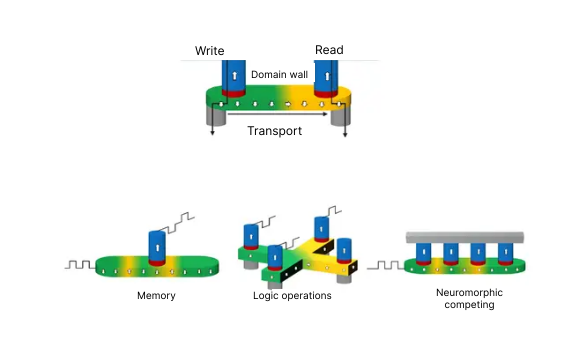
\includegraphics[width=0.75\textwidth]{Figures/mram.png}
    \caption{ Magnetic Random Memories }
    \label{fig:skyrmions_textures}
\end{figure}


b) Magnetic nanoparticles are used in oncological hyperthermia therapies, drug targeting, and enhanced magnetic resonance imaging (MRI). Their efficiency depends on the dynamic spin response under alternating fields, which is determined by the internal structure and anisotropy of the material \cite{Barrera2023, IronOxideReview2023, MLDesign2023}.


\begin{figure}[H]
    \centering
    \includegraphics[width=0.75\textwidth]{Figures/medicine.jpg}
    \caption{ Biomedical applications }
    \label{fig:skyrmions_textures}
\end{figure}

c) Energy Conversion and Storage. In the energy field, magnetic nanoparticles are
investigated for magnetocaloric refrigeration, thermoelectric conversion, and magnetic
energy storage \cite{He2025, Nehan2024, Hadouch2022}. The spin configurations determine
the mechanisms of energy transfer between magnetic and thermal degrees of freedom,
directly influencing the efficiency of these processes \cite{Liedienov2021, Nehan2024}.


\begin{figure}[H]
    \centering
    \includegraphics[width=0.45\textwidth]{Figures/storage.png}
    \caption{ Biomedical applications }
    \label{fig:skyrmions_textures}
\end{figure}





%2.4 Scientific Importance of Nanoscale Studies

The analysis of magnetic systems at the nanoscale not only drives the development of new technologies but also contributes fundamental knowledge about emergent phenomena in condensed matter physics \cite{Xiao2023, Liao2023}. These systems serve as natural models of complex physical behavior, where local interactions give rise to collective responses that challenge classical linear approximations \cite{Xiao2023, DeepSPIN2023}.

In recent years, the integration of Artificial Intelligence (AI) with computational physics has opened new avenues for the modeling and prediction of complex material behaviors \cite{Hilgers2025, Ryu2025, Goswami2022}. Traditional simulation methods offer precise control over physical parameters but are limited by high computational cost and restricted scalability across parameter spaces \cite{Liao2023}. AI-driven approaches, particularly deep learning architectures, enable the extraction of latent physical relationships directly from data, accelerating the exploration of vast configuration spaces that would otherwise be computationally intractable \cite{Xiao2023, Hilgers2025}. When coupled with physics-informed principles, these models not only enhance predictive accuracy but also preserve interpretability and physical consistency \cite{Ryu2025, Sharma2023}. In the context of nanoscale magnetism, such hybrid frameworks bridge the gap between experimental observation and theoretical modeling, providing a data-efficient path toward inverse design and the discovery of emergent spin phenomena \cite{DeepSPIN2023, Liao2023}.


\vspace{0.5cm}
%%% PARRAFO CON RELACIÓN A GCPDS
%%%
%%% REFERENCIAS DEL GRUPO?
%%%
This work is developed within the Research Signal Processing and Recognition  (GCPDS), which has extensive experience in the design and implementation of intelligent systems for signal and image analysis. The group has explored artificial intelligence methodologies across multiple domains, including image processing, temporal series analysis, and, more recently, electroencephalographic (EEG) signal interpretation. Building on this background, GCPDS is currently expanding its research toward the application of AI in computational physics, focusing on the intersection between data-driven learning and physical modeling. Current efforts involve the integration of generative models, interpretability mechanisms, transformer-based architectures, and optimization strategies to develop hybrid frameworks capable of revealing underlying physical principles from complex experimental data. This interdisciplinary approach establishes a foundation for applying advanced machine learning to the understanding and design of magnetic systems at the nanoscale. %% PAULINA


\section{Problem Statement}
%%%% Experimental and Theoretical Approaches to Magnetic Nanostructures
 
The study of magnetic nanostructures integrates two complementary approaches: the \textbf{experimental} and the \textbf{theoretical-simulation} pathways \cite{Streubel2022}. The experimental route focuses on the physical synthesis, visualization, and measurement of magnetic systems \cite{Zhang2024MFM, Wiesendanger2022SPSTM}, whereas the theoretical approach aims to model and predict their magnetic behavior from first principles or phenomenological descriptions \cite{Evans2014Atomistic, MuMaxReview2021}.


From the experimental perspective, research begins with the \textit{sample preparation} of thin films, multilayers, or nanostructures that define the system’s geometry and magnetic anisotropy \cite{Nagaosa2021Deposition, Fert2022ThinFilms}. These samples are then characterized through advanced \textit{magnetic imaging techniques} such as Lorentz Transmission Electron Microscopy (TEM), Magnetic Force Microscopy (MFM), and Kerr microscopy, which reveal the domain patterns at nanometer resolution \cite{Streubel2022, Zhang2024MFM, McVitie2023Lorentz}. The resulting data are complemented by \textit{acquisition and analysis} of external stimuli, including magnetic and electric fields (STT and SOT effects), strain fields, and temperature variations, which allow for the control and manipulation of domain structures \cite{Manchon2019SOT, Yu2022StrainControl, Finco2024Stimuli}.


In parallel, the theoretical and computational approach seeks to describe these systems at different scales. At the \textit{atomistic level}, models such as the Heisenberg Hamiltonian and Monte Carlo simulations capture spin interactions with atomic precision \cite{Evans2014Atomistic, Nowak2007MC, Hinzke2022Atomistic}. Moving to larger scales, \textit{micromagnetic simulations} employ the Landau–Lifshitz–Gilbert (LLG) equation to model the continuous magnetization field, implemented through frameworks like MuMax3, OOMMF, and Spirit \cite{MuMaxReview2021, Donahue1999OOMMF, Spirit2020}.

Together, these methodologies constitute a multi-scale, multi-modal ecosystem that bridges empirical observation and theoretical understanding, providing the foundation for modern research in magnetic materials \cite{Gomez2023MultiscaleReview}.



\begin{figure}[H]
    \centering
    \includegraphics[width=0.75\textwidth]{Figures/ProblemStatement.png}
    \caption{ Magnetic Domain Approach }
    \label{fig:skyrmions_textures}
\end{figure}

From an experimental perspective, advances in Magnetic Force Microscopy (MFM) and Spin-Polarized Scanning Tunneling Microscopy (SP-STM) have enabled direct visualization of nanoscale magnetic textures, revealing complex domain morphologies such as vortices, skyrmions, and labyrinthine patterns \cite{Zhang2024MFM, Wiesendanger2022SPSTM, McVitie2023Lorentz}. However, experimental images often contain noise, contrast distortions, and limited resolution, making quantitative parameter extraction challenging \cite{Gao2021NoiseMFM, Phark2022ResolutionLimits}. As a result, bridging the gap between simulated and observed magnetic configurations remains an open problem that hinders both predictive modeling and materials discovery \cite{Liao2023, DeepSPIN2023, Finco2024Stimuli}.


%%%%%%%%%%%%%%%%%%%%%%%%%%%%%%%%%%%%%%%%%%%%%%%%%%%%%%%%%%
%%% EXTENSIÓN PARA HABLAR DE LAS SIMULACIONES Y PROBLEMAS 
%%%%%%%%%%%%%%%%%%%%%%%%%%%%%%%%%%%%%%%%%%%%%%%%%%%%%%%%%%
Despite the significant advances in atomistic and micromagnetic simulations, the theoretical–computational approach faces several inherent limitations that restrict its scalability and practical applicability. First, the computational cost associated with solving high-dimensional Hamiltonian systems grows rapidly with the number of spins and spatial resolution, making large-scale or time-dependent studies computationally prohibitive \cite{Gomes2022Limitations, Hinzke2022Atomistic}. Parameter sweeps over exchange coupling, anisotropy, or Dzyaloshinskii–Moriya interaction (DMI) often require thousands of independent simulation runs, each demanding considerable processing time and memory resources \cite{Gomez2023MultiscaleReview, MuMaxReview2021}, and the approximation level of each simulation method imposes constraints on physical fidelity \cite{Nowak2007MC, Evans2014Atomistic}. Atomistic models offer high precision but are limited to small systems, while micromagnetic models extend spatial coverage at the expense of losing atomistic detail \cite{Spirit2020, McMichael2009Limitations}. Incorporating temperature effects, stochastic fluctuations, and material imperfections further increases complexity and reduces interpretability \cite{Hinzke2022Atomistic, Brown1963Thermal}.  



%%%%%%%%%%%%%%%%%%%%%%%%%%%%%%%%%%%%%%%%%%%%%%
% INTRODUCCIÓN AL PROBLEMA INVERSO Y DIRECTO %
%%%%%%%%%%%%%%%%%%%%%%%%%%%%%%%%%%%%%%%%%%%%%%
Within this integrated context, the study of magnetic nanostructures can be framed around two complementary and interdependent challenges: the direct and the inverse magnetic domain problems \cite{Feng2024, Liao2023}.

The direct problem involves predicting or generating the magnetic domain configuration that emerges from a given set of Hamiltonian parameters—exchange interaction, anisotropy, DMI, external magnetic field, and temperature. This process defines the forward mapping from the parameter space to the spatial magnetization distribution and is typically addressed using micromagnetic or atomistic simulations \cite{Evans2014Atomistic, MuMaxReview2021, Nowak2007MC}. However, such simulations are often computationally intractable for broad parameter exploration or for incorporating stochastic thermal and experimental effects \cite{Gomes2022Limitations, Hinzke2022Atomistic, Brown1963Thermal}.


\begin{figure}[H]
    \centering
    \includegraphics[width=0.75\textwidth]{Figures/Direct.png}
    \caption{ Magnetic Domain Approach }
    \label{fig:skyrmions_textures}
\end{figure}

In contrast, the inverse problem aims to infer the underlying physical parameters responsible for a given observed domain configuration, such as those obtained from Magnetic Force Microscopy (MFM) or Spin-Polarized Scanning Tunneling Microscopy (SP-STM) \cite{Zhang2024MFM, Wiesendanger2022SPSTM}. This task is intrinsically ill-posed: multiple parameter combinations can reproduce visually similar textures, leading to degeneracy and uncertainty in parameter estimation \cite{Feng2024, Liu2023, DeepSPIN2023}.


\begin{figure}[H]
    \centering
    \includegraphics[width=0.75\textwidth]{Figures/Inverse.png}
    \caption{ Magnetic Domain Approach }
    \label{fig:skyrmions_textures}
\end{figure}

Bridging these two directions—ensuring coherence between generation (direct mapping) and estimation (inverse mapping)—is essential for predictive materials discovery \cite{Feng2024, Park2024}. A unified and physically consistent framework that can simultaneously learn both directions offers a pathway toward explainable, data-driven modeling of nanoscale magnetic phenomena \cite{DeepSPIN2023, Ryu2025, Hilgers2025}.

Overall, the study of magnetic nanodots is constrained by three fundamental challenges that motivate the development of hybrid approaches combining physical modeling and data-driven inference \cite{Gomez2023MultiscaleReview, Liao2023, Evans2014Atomistic}.



\begin{figure}[H]
\centering
\begin{adjustbox}{center, max width=\textwidth}
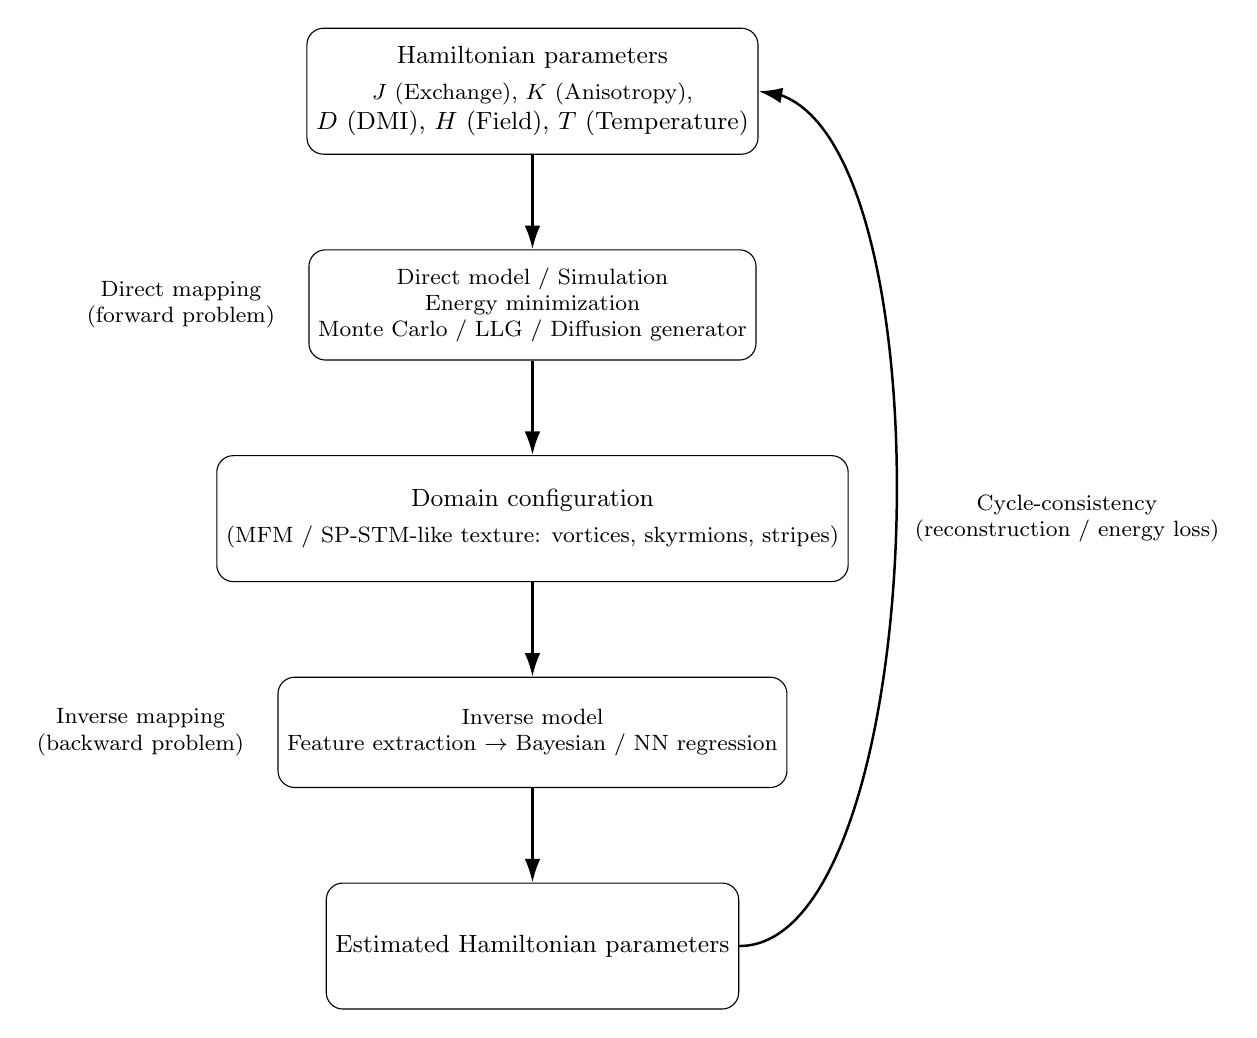
\begin{tikzpicture}[
  box/.style = {draw, rounded corners=6pt, minimum width=5cm, minimum height=1.6cm, align=center, font=\small},
  process/.style = {draw, rounded corners=6pt, minimum width=5cm, minimum height=1.4cm, align=center, font=\footnotesize},
  arr/.style = {-{Latex[length=3mm,width=2mm]}, line width=0.9pt},
  dashedarr/.style = {->, dashed, line width=0.9pt},
  node distance=12mm
]

% --- Nodes (top to bottom) ---
\node[box] (ham) {Hamiltonian parameters\\[2pt]
\footnotesize $J$ (Exchange), $K$ (Anisotropy),\\ $D$ (DMI), $H$ (Field), $T$ (Temperature)};

\node[process, below=of ham] (direct) {Direct model / Simulation\\
\footnotesize Energy minimization \\ Monte Carlo / LLG / Diffusion generator};

\node[box, below=of direct] (domain) {Domain configuration\\[2pt]
\footnotesize (MFM / SP-STM-like texture: vortices, skyrmions, stripes)};

\node[process, below=of domain] (inverse) {Inverse model \\ \footnotesize Feature extraction $\rightarrow$ Bayesian / NN regression};

\node[box, below=of inverse] (est) {Estimated Hamiltonian parameters};

% --- Arrows ---
\draw[arr] (ham) -- (direct);
\draw[arr] (direct) -- (domain);
\draw[arr] (domain) -- (inverse);
\draw[arr] (inverse) -- (est);

% --- Loop arrow back up (cycle consistency) ---
\draw[arr] (est.east) .. controls +(2.5,0) and +(2.5,0) .. (ham.east)
node[midway, right=1mm, font=\footnotesize, align=center] {Cycle-consistency\\(reconstruction / energy loss)};

% --- Labels ---
\node[font=\footnotesize, align=center, left=3mm of direct] {Direct mapping\\(forward problem)};
\node[font=\footnotesize, align=center, left=3mm of inverse] {Inverse mapping\\(backward problem)};

\end{tikzpicture}
\end{adjustbox}
\caption{Vertical unified cycle illustrating the direct (top-down) and inverse (bottom-up) problems in magnetic domain research. The cycle-consistency loop (right) enforces physical coherence between estimated Hamiltonian parameters and generated magnetic textures.}
\label{fig:vertical-cycle}
\end{figure}



Overall, the study of magnetic nanodots is constrained by three fundamental challenges that motivate the development of hybrid approaches combining physical modeling and data-driven inference:

\vspace{0.5cm}

\subsection{Degeneracy of Magnetic States}
%% ACORTAR EL TITULO DEL PROBLEM STATEMTN --CHECK
%% INTERPRETABILIDAD INCLUYENDO RESTRICCIONES FISICAS.

%% MODELO FISICO PARA SOPORTAR POCOS DATOS
%% TEMATICO DE RUIDO.

%% QUESTIÓN.  CON EL TITULO Y EL OBJETIVO GENERAL
%% DEBE QUEDAR CLARO LA PALABRA O MAXIMO 2 PALABRAS CLAVE DE LOS 3 PROBLEMAS.

%% MIRAR EL VIERNES

\vspace{0.5cm}

Different combinations of Hamiltonian parameters—such as exchange interaction, anisotropy, and Dzyaloshinskii–Moriya interaction (DMI)—can lead to visually similar magnetic patterns \cite{Feng2024, Liao2023, DeepSPIN2023}. This degeneracy complicates the unique identification of physical parameters from experimental observations, creating ambiguity in inverse estimation tasks \cite{Park2024, Liu2023InverseML, Raju2022SkyrmionInverse}.


\begin{figure}[H]
    \centering
    \includegraphics[width=0.45\textwidth]{Figures/Problems1.png}
    \caption{Degenerate magnetic states arising from distinct parameter combinations.}
    \label{fig:degeneracy_problem}
\end{figure}

In nanoscale magnetic systems, the relationship between the Hamiltonian parameters and the resulting domain configurations is highly nonlinear and often degenerate \cite{Feng2024, Liao2023}. This degeneracy arises because different combinations of exchange coupling (J), magnetic anisotropy (K), and Dzyaloshinskii–Moriya interaction (D) can produce equilibrium states with similar total energy and comparable spatial magnetization patterns \cite{Raju2022SkyrmionInverse, DeepSPIN2023}. From a physical perspective, the energy landscape of the magnetic Hamiltonian contains multiple local minima corresponding to metastable spin textures—such as vortices, skyrmions, or labyrinthine domains—that can be stabilized under different parameter sets \cite{Leonov2020EnergyLandscape, Du2022MetaStableSkyrmions}. In practice, this means that small compensations between parameters can preserve the overall balance of competing interactions: for example, an increase in anisotropy can be offset by a stronger exchange term or a weaker DMI, yielding morphologically indistinguishable configurations \cite{Liu2023InverseML, Bessarab2018EnergyBarriers}. Thermal fluctuations and boundary effects further blur these distinctions by allowing transitions between nearby minima, effectively broadening the range of parameter combinations that generate similar observable textures \cite{Hertel2023Thermal, Maletta2021BoundaryEffects}. As a result, the mapping from physical parameters to domain patterns is non-injective, complicating the inverse identification of Hamiltonian parameters from experimental images and introducing intrinsic ambiguity in inverse modeling tasks \cite{Park2024, Ryu2025}.


\begin{figure}[H]
    \centering
    \includegraphics[width=0.8\textwidth]{Figures/NonUniqueness.png}
    \caption{Energy Landscape of magnetic hamiltonian}
    \label{fig:degeneracy_problem}
\end{figure}


\subsection{Low Quality Data}
Magnetic domain imaging and modeling face intrinsic limitations that affect the quality
and reliability of observable data. On the experimental side, characterization techniques
such as Magnetic Force Microscopy (MFM) and Spin-Polarized Scanning Tunneling
Microscopy (SP-STM) provide direct access to nanoscale magnetic textures but are
fundamentally constrained by instrumental noise, finite probe resolution, and contrast
distortions \cite{Schlenhoff2022SPSTM, Kramer2021MFMNoise, Raabe2020ImagingLimits}. These imperfections obscure the fine spatial structure of the magnetization
field, complicating the quantitative extraction of physical parameters and domain wall
profiles \cite{Hanneken2022ResolutionLimit, Wiesendanger2023SPSTMReview}. On the computational side, numerical simulations—whether atomistic or
micromagnetic—introduce their own forms of degradation. Discretization errors in
the mesh, finite time-step integration of the Landau–Lifshitz–Gilbert (LLG) dynamics,
and simplifications in boundary or anisotropy conditions limit the accuracy of the
resulting spin configurations \cite{Evans2014Atomistic, Exl2021NumericalErrors, Hertel2022MicromagneticLimits}. As a result, both experimental and simulated datasets
often represent only approximations of the true magnetic state, making the comparison
between observed and modeled textures inherently uncertain \cite{Liao2023, Park2024}.


\begin{figure}[H]
    \centering
    \includegraphics[width=0.45\textwidth]{Figures/Lab.png}
    \caption{Experimental observation limitations due to noise and resolution constraints.}
    \label{fig:experimental_limitations}
\end{figure}

\begin{table}[H]
\centering
\caption{Approximate operational costs and limitations of magnetic imaging techniques.}
\label{tab:experimental_costs_monetary}
\renewcommand{\arraystretch}{2}
\large
\resizebox{\textwidth}{!}{
\begin{tabular}{lcccc}
\hline
\textbf{Technique} & \textbf{Spatial Resolution} & \textbf{Main Limitations} & \textbf{Quantitative Accuracy} & \textbf{Estimated Cost (USD/hour)} \\ \hline
Magnetic Force Microscopy (MFM) & 30–50 nm & Tip-induced artifacts, long scan time & Moderate & 150–300 \\
Spin-Polarized STM (SP-STM) & $\sim$1 nm & Requires UHV and cryogenic conditions & High (atomic-level) & 800–1500 \\
Lorentz Transmission Electron Microscopy (Lorentz TEM) & 5–10 nm & Complex sample prep, projection effects & Moderate–High & 400–800 \\
Kerr Microscopy & 300–500 nm & Optical diffraction limit, surface sensitivity & Low–Moderate & 100–250 \\
X-ray Magnetic Circular Dichroism (XMCD) & 10–30 nm & Requires synchrotron access & High & 2000–5000 \\
Electron Holography & 2–5 nm & High vacuum, phase noise & High & 500–1000 \\ \hline
\end{tabular}
}
\end{table}


From a physical standpoint, this degradation is a direct manifestation of the multi-
scale and metastable nature of magnetic systems. The magnetic free-energy landscape
is rugged, containing multiple nearby minima separated by small energy barriers \cite{Leonov2020EnergyLandscape, Bessarab2018EnergyBarriers}. Even
slight variations in temperature, defects, or external fields can cause the system to
relax into different local minima that are energetically similar but structurally distinct \cite{Du2022MetaStableSkyrmions, Hertel2023Thermal}. Consequently, any measurement or simulation captures only one realization of a broader
ensemble of possible states. In experimental observations, this variability is further
blurred by the indirect nature of detection: instruments like MFM record the stray field
above the surface, which is a convolution of the probe’s sensitivity and the sample’s
magnetization, rather than a direct mapping of the spin structure itself \cite{Kramer2021MFMNoise, Raabe2020ImagingLimits}. Similarly, in
simulations, numerical smoothing and discretization coarsen the magnetization field,
suppressing high-frequency details \cite{Exl2021NumericalErrors, Hertel2022MicromagneticLimits}. Together, these effects impose a fundamental limit
on the fidelity of both experimental and computational data, constraining the precision
of parameter estimation and the interpretability of magnetic textures \cite{Liao2023, Park2024}.



\begin{figure}[H]
    \centering
    \includegraphics[width=0.97\textwidth]{Figures/Sensitive.png}
    \caption{Experimental observation limitations due to noise and resolution constraints.}
    \label{fig:experimental_limitations}
\end{figure}

\subsection{Lack of physic-based interpretability}
A persistent challenge in data-driven modeling of magnetic systems is the lack of in-
terpretability and physical traceability in the results. While modern machine learning
methods can efficiently approximate the complex mapping between Hamiltonian pa-
rameters and magnetic domain configurations, their internal representations are often
opaque, providing limited insight into the underlying physics that govern the observed
phenomena \cite{Rao2022ExplainableMaterialsML, Park2024, DeepSPIN2023}. This opacity complicates the validation of learned relationships against es-
tablished physical laws, such as exchange symmetry, anisotropy effects, or DMI-induced
chirality \cite{Chen2021PINNMagnetism, Ryu2025, Schneider2022MLMagnetism}. Furthermore, when combined with noisy experimental data or degenerate
parameter spaces, black-box models may produce accurate reconstructions without
preserving causal or physically meaningful dependencies \cite{Liao2023, Liu2023InverseML}. Consequently, the absence
of interpretability not only limits the scientific reliability of such approaches but also
hinders their use in guiding material design and hypothesis generation \cite{Butler2018MLMaterials, Sanchez2023ExplainableDesign}. Bridging this
gap requires the integration of physics-informed constraints, explainable architectures,
and cycle-consistent frameworks that ensure alignment between learned representations
and physically observable quantities \cite{Karniadakis2021PINNs, Sanchez2024CycleConsistentMaterials}.

\begin{figure}[H]
    \centering
    \includegraphics[width=0.45\textwidth]{Figures/Interpretability.png}
    \caption{Interpretability Challenges}
    \label{fig:experimental_limitations}
\end{figure}

The three outlined challenges---parameter degeneracy, data degradation, and lack of interpretability---are deeply interconnected within the study of magnetic domain systems \cite{Feng2024, Exl2021NumericalErrors, Rao2022ExplainableMaterialsML}. Parameter degeneracy reflects the intrinsic non-uniqueness of the physical mapping between Hamiltonian parameters and magnetic configurations, producing multiple metastable states with similar energy and morphology \cite{Leonov2020EnergyLandscape, Du2022MetaStableSkyrmions}. Data degradation, in turn, limits the quality and reliability of both experimental and simulated observations, as noise, instrumental artifacts, and numerical discretization blur the underlying spin structures \cite{Kramer2021MFMNoise, Exl2021NumericalErrors, Raabe2020ImagingLimits}. Finally, the lack of interpretability in data-driven models prevents the extraction of causal or physically meaningful relationships from these imperfect datasets, reducing their scientific value and applicability \cite{Park2024, Chen2021PINNMagnetism, Sanchez2023ExplainableDesign}. Together, these issues define a complex landscape where conventional simulation-based approaches struggle with scalability and uncertainty, while purely data-driven models risk overfitting and opacity \cite{Gomez2023MultiscaleReview, Butler2018MLMaterials, Ryu2025}. This convergence of physical ambiguity, informational degradation, and epistemic opacity motivates the development of hybrid, physics-informed frameworks capable of enforcing physical consistency while enabling explainable inference across the direct and inverse magnetic domain problems \cite{Karniadakis2021PINNs, DeepSPIN2023, Sanchez2024CycleConsistentMaterials}.

\bigskip




%


%



%
\section{State of the art}

\noindent
The study of magnetic domain systems has evolved through complementary experimen-
tal, theoretical, and computational approaches, each contributing to the understanding
of spin textures and their emergent phenomena \cite{Wiesendanger2023SPSTMReview, Gomez2023MultiscaleReview}. Recent advances in high-resolution
imaging techniques, micromagnetic simulations, and machine learning frameworks have
expanded the capacity to visualize, model, and predict complex domain morphologies
such as skyrmions, vortices, and labyrinthine structures \cite{Hanneken2022ResolutionLimit, Hertel2022MicromagneticLimits, DeepSPIN2023}. However, despite the increasing
sophistication of these methodologies, several fundamental challenges persist that con-
strain the reliability, interpretability, and generalization of current models \cite{Feng2024, Exl2021NumericalErrors, Rao2022ExplainableMaterialsML}. Specifically,
three major issues remain at the core of contemporary research: (i) the degeneracy of
the Hamiltonian parameter space, which complicates inverse estimation and physical
uniqueness \cite{Liao2023, Raju2022SkyrmionInverse}; (ii) the degradation of data quality in both experimental and simulated
observations, which limits quantitative analysis \cite{Kramer2021MFMNoise, Raabe2020ImagingLimits}; and (iii) the lack of interpretability in
data-driven approaches, which obscures causal understanding and hinders physics-based
validation \cite{Park2024, Sanchez2023ExplainableDesign}. The following subsections review the main advances and limitations related
to each of these challenges, outlining the current research gaps that motivate the present
work.



\subsection{Degeneracy of Magnetic States}


The degeneracy of magnetic states represents one of the most persistent obstacles in the modeling, interpretation, and inverse reconstruction of spin textures. This phenomenon arises because the magnetic free-energy landscape is intrinsically multimodal, admitting a large number of metastable solutions whose morphology can be remarkably similar even when generated by substantially different Hamiltonian parameters \cite{Leonov2020EnergyLandscape, Bessarab2018EnergyBarriers}. As a consequence, both the direct problem (mapping parameters to imaging contrast) and the inverse problem (inferring parameters from an observed texture) are fundamentally ill-posed. The state of the art has therefore evolved along two complementary lines of work: efforts to make the forward mapping more discriminative and physically grounded, and efforts to make the inverse mapping more expressive, uncertainty-aware, and physically constrained. What follows is a synthesis of the major developments, their strengths and limitations, and the structural gaps that motivate new approaches.

Research on the direct problem has traditionally relied on high-fidelity micromagnetic or atomistic simulations capable of capturing the subtle competition between exchange, anisotropy, DMI, dipolar interactions, and applied fields. Tools such as MuMax3, OOMMF, and Spirit have enabled precise modeling of domain walls, skyrmions, vortices, and labyrinthine patterns under a wide range of physical conditions \cite{MuMaxReview2021, Spirit2020}. When combined with forward-rendering models that explicitly account for experimental transfer functions—such as the point-spread function of an MFM tip, the convolution biases of SP-STM, or noise due to feedback electronics—these simulators can generate synthetic images that closely resemble those obtained experimentally \cite{Kramer2021MFMNoise, Phark2022ResolutionLimits}. Such physically accurate models improve the discriminability of parameter changes and help reduce trivial degeneracies that arise purely from inadequate instrument modeling.

Nevertheless, these simulator-based approaches are computationally expensive and sensitive to numerical discretization, initialization conditions, and solver choices. Moreover, even perfect simulations cannot eliminate intrinsic degeneracy: two or more sets of Hamiltonian parameters may legitimately give rise to nearly indistinguishable magnetic textures, making the direct mapping inherently non-injective. Thus, while improved simulators help expose the structure of degeneracy in parameter space, they do not resolve it.

To mitigate these problems, recent work has turned to differentiable and surrogate forward models. Neural surrogates, variational approximators, and differentiable micromagnetic solvers provide orders-of-magnitude speedups and enable gradient-based calibration and integration into larger learning frameworks \cite{Kwon2020, DeepSPIN2023}. Their efficiency makes it possible to explore high-dimensional parameter spaces and embed forward models within Bayesian pipelines. However, their accuracy depends on the representativeness of the simulation data used during training, and they may inadvertently hallucinate non-physical textures or fail to generalize beyond the training domain. These surrogates often interpolate well but extrapolate poorly, revealing a structural gap in the field: the lack of certified, physics-faithful differentiable simulators that reliably preserve the constraints and symmetries of the underlying micromagnetic equations.

Parallel to these developments, physics-informed neural networks (PINNs) and hybrid modeling frameworks have gained traction by embedding the Landau–Lifshitz–Gilbert (LLG) equation or energetic constraints directly into the learning objective \cite{Karniadakis2021PINNs, Chen2021PINNMagnetism}. Such approaches improve the physical plausibility of generated textures and restrict the feasible mapping from parameters to images, thereby narrowing the set of degenerate solutions. Nevertheless, PINNs for magnetic systems remain difficult to train due to the stiffness of the LLG equation and the challenges of balancing physical losses with data-driven objectives. Their scalability to realistic films, finite-temperature regimes, and domain geometries remains an open research challenge.


The use of conditional generative models—including conditional VAEs and GANs has introduced a qualitatively different perspectiv. These models treat the forward mapping as a conditional distribution rather than a deterministic function, enabling them to represent multimodality explicitly \cite{Ronne2024, Alverson2024, Chen2024}. They can generate multiple plausible images for a single parameter set, thereby sampling the degeneracy rather than attempting to collapse it. Yet generative models tend to lack strict physical guarantees unless coupled with physics-based regularizers or energy-informed discriminators. Their fidelity and physical consistency vary widely across architectures, and there is currently no benchmark for evaluating their agreement with micromagnetic ground truth.

\begin{figure}[H]
\centering
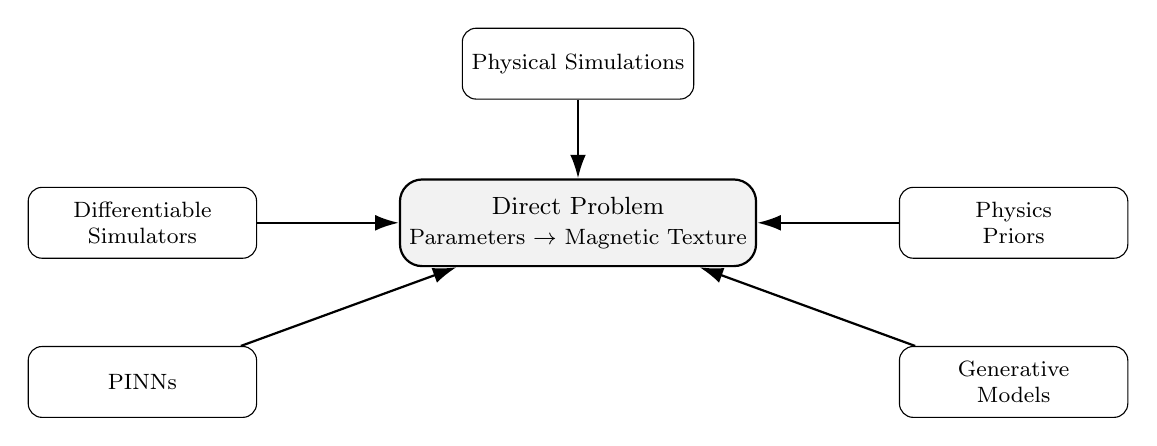
\begin{tikzpicture}[
  node distance=10mm and 16mm,
  box/.style={
    draw, rounded corners=5pt,
    minimum width=2.9cm,
    minimum height=0.9cm,
    align=center,
    font=\footnotesize,
    fill=white
  },
  centerbox/.style={
    draw, rounded corners=8pt, thick,
    minimum width=3.4cm,
    minimum height=1.1cm,
    align=center,
    font=\small,
    fill=gray!10
  },
  arrow/.style={-{Latex[length=3mm,width=2mm]}, thick}
]

% CENTERED MAIN NODE
\node[centerbox] (core) {Direct Problem\\ \footnotesize Parameters $\rightarrow$ Magnetic Texture};

% --- SYMMETRIC NODES (manually aligned) ---
\node[box, above=of core]            (phys)  {Physical Simulations};
\node[box, left=of core, xshift=-2mm] (diff)  {Differentiable\\ Simulators};
\node[box, right=of core, xshift=2mm] (priors){Physics\\ Priors};
\node[box, below left=of core, xshift=-2mm] (pinns) {PINNs};
\node[box, below right=of core, xshift=2mm] (gen)   {Generative\\ Models};

% SYMMETRIC ARROWS
\draw[arrow] (phys) -- (core);
\draw[arrow] (diff) -- (core);
\draw[arrow] (priors) -- (core);
\draw[arrow] (pinns) -- (core);
\draw[arrow] (gen) -- (core);

\end{tikzpicture}
\caption{Compact conceptual map for the direct problem (Hamiltonian parameters $\rightarrow$ magnetic texture).}
\end{figure}


On the inverse side, early approaches framed parameter estimation as a supervised regression problem, with convolutional or fully connected networks trained on large synthetic datasets \cite{Kwon2020, Feng2024}. Although such models can infer parameters extremely rapidly, they collapse ambiguity into a single point estimate and are highly sensitive to both sim-to-exp mismatch and dataset bias. Whenever two or more parameter regimes generate indistinguishable images, these models tend to produce unstable or misleading predictions. Their reliance on large, representative datasets introduces a dependency on simulator quality and coverage, which remains a critical bottleneck.

The limitations of strict regression have motivated a shift toward Bayesian inference methodologies, which represent the inverse mapping as a posterior distribution rather than a deterministic estimate \cite{Hu2025, PRMaterials2025_phaseboundaries}. By explicitly modeling uncertainty and multimodality, Bayesian frameworks expose the underlying degeneracy rather than hiding it. They provide distributions over parameter space that reflect both physical ambiguity and measurement uncertainty. However, full Bayesian inference is computationally demanding because it requires repeated forward evaluations—each potentially involving a micromagnetic simulation or a complex surrogate. Moreover, posterior accuracy depends strongly on the quality of the likelihood model and the choice of prior, both of which are notoriously difficult to define in micromagnetism.

A particularly promising direction lies in cycle-consistent frameworks, which couple a forward surrogate and an inverse estimator and enforce that each is consistent with the other \cite{DeepSPIN2023, Sanchez2024CycleConsistentMaterials}. By requiring that parameters inferred from an image can regenerate that image through the forward model, these methods eliminate many non-physical or inconsistent solutions. Yet cycle consistency also inherits any biases or inaccuracies present in the forward surrogate, and if poorly designed, it may reinforce rather than mitigate systematic errors. The stability of cycle-consistent training for micromagnetic problems remains poorly understood, representing another gap in the literature.

Finally, hybrid inverse methods that incorporate physics-based priors, energy regularization, or LLG residual penalties have shown promise in preventing non-physical parameter estimates. Bayesian PINNs and energy-constrained inverse networks can restrict inference to regions of parameter space that are physically interpretable and energetically plausible \cite{Chen2021PINNMagnetism, Ryu2025}. These approaches improve interpretability, but at the cost of increased computational complexity and difficult-to-sample posteriors, particularly in the presence of strong multimodality.

\begin{figure}[H]
\centering
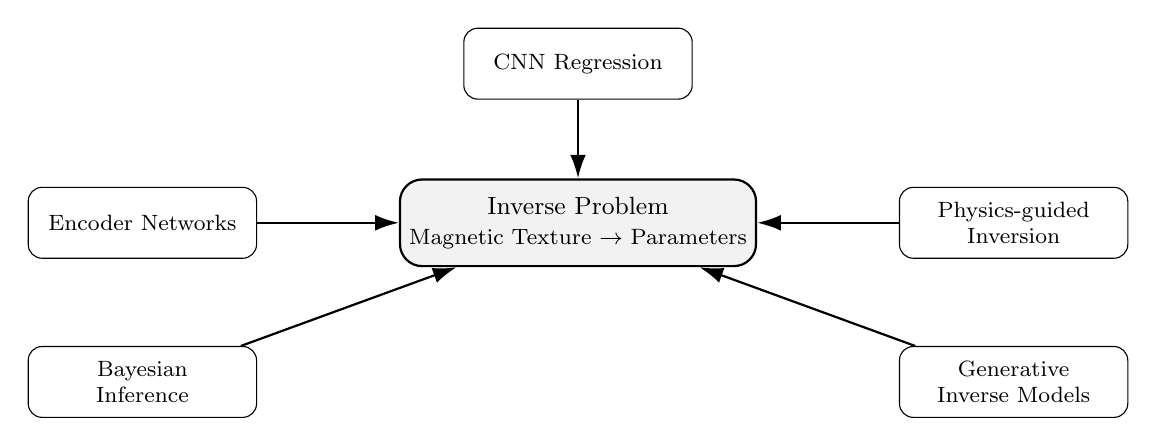
\begin{tikzpicture}[
  node distance=10mm and 16mm,
  box/.style={
    draw, rounded corners=5pt,
    minimum width=2.9cm,
    minimum height=0.9cm,
    align=center,
    font=\footnotesize,
    fill=white
  },
  centerbox/.style={
    draw, rounded corners=8pt, thick,
    minimum width=3.4cm,
    minimum height=1.1cm,
    align=center,
    font=\small,
    fill=gray!10
  },
  arrow/.style={-{Latex[length=3mm,width=2mm]}, thick}
]

% CENTER NODE
\node[centerbox] (core) {Inverse Problem\\ \footnotesize Magnetic Texture $\rightarrow$ Parameters};

% SYMMETRIC PERIPHERAL NODES
\node[box, above=of core]                           (cnn)   {CNN Regression};
\node[box, left=of core, xshift=-2mm]               (enc)   {Encoder Networks};
\node[box, right=of core, xshift=2mm]               (inv)   {Physics-guided\\ Inversion};
\node[box, below left=of core, xshift=-2mm]         (bay)   {Bayesian\\ Inference};
\node[box, below right=of core, xshift=2mm]         (gen)   {Generative\\ Inverse Models};

% ARROWS
\draw[arrow] (cnn) -- (core);
\draw[arrow] (enc) -- (core);
\draw[arrow] (inv) -- (core);
\draw[arrow] (bay) -- (core);
\draw[arrow] (gen) -- (core);

\end{tikzpicture}
\caption{Compact conceptual map for the inverse problem (magnetic texture $\rightarrow$ Hamiltonian parameters).}
\end{figure}


Despite these advances, several structural gaps persist within the state of the art. Foremost among them is the absence of standardized benchmarks that rigorously evaluate the fidelity, uncertainty calibration, and physical consistency of forward and inverse models across multiple geometries and experimental conditions. Likewise, there is no established methodology for quantifying numerical uncertainty in micromagnetic solvers or propagating such uncertainty to inverse predictions. The lack of certified differentiable simulators, combined with limited understanding of surrogate-induced biases, hampers progress toward robust inverse methods. Moreover, current approaches rarely integrate physical constraints, uncertainty quantification, and cycle-consistent learning within a unified architecture capable of handling both direct and inverse degeneracy in a principled manner.



\subsection{Low-Quality Data}

The quality of magnetic-domain images (MFM, SP-STM, Kerr, Lorentz TEM, etc.) critically conditions both forward modeling and inverse inference. Experimental images often suffer from low signal-to-noise ratio (SNR), probe convolution, contrast distortions, finite spatial resolution and sample variability; numerical datasets produced by simulators can display different noise statistics and missing instrumental effects. These issues produce two distinct but related failure modes: (i) loss of physically informative fine structure (domain walls, skyrmion cores), which degrades parameter identifiability; and (ii) domain shift between simulation and experiment, which causes learned models to generalize poorly. The recent literature addresses these problems through a set of complementary strategies: denoising and super-resolution (including zero-shot/self-supervised methods), domain adaptation / transfer learning (sim2real), physics-informed reconstruction (PINNs and physics-regularized denoisers), instrument modelling and deconvolution, and generative priors used as reconstructors or regularizers. Below we summarize each approach, list strengths/weaknesses, and point out explicit gaps that motivate further work.

\paragraph{Denoising and super-resolution (classical and deep learning).}  
Deep denoising and single-image super-resolution methods are applied to recover fine spatial details necessary for physical interpretation (sharp domain walls, core polarity). Supervised CNNs and residual networks trained on paired synthetic noisy/clean images achieve excellent reconstruction when training data matches test conditions, while self-supervised and zero-shot methods (e.g., Noise2Void, Noise2Self, zero-shot SR) enable enhancement without paired HR/LR datasets, a crucial advantage when experimental ground truth is scarce \cite{Noise2Void2019, SelfSuper2020, PMC11230634}. The main risk is over-smoothing or creation of hallucinated features that do not correspond to actual magnetization structure; supervised models trained on synthetic physics outputs can introduce domain-specific artefacts if instrument effects are mismatched.

\paragraph{Domain adaptation.}  
Bridging the simulation–experiment gap is commonly addressed through domain adaptation and transfer learning: fine-tuning networks on a (small) set of real images, adversarial domain adaptation to align feature distributions, and test-time adaptation techniques that adapt model statistics on the fly. These techniques reduce the performance drop when deploying inverse regressors on experimental images, but they require at least some representative real data or reliable unsupervised adaptation heuristics; moreover, they cannot correct for unmodelled physical differences (e.g., unknown tip magnetization, unknown boundary roughness) \cite{Sim2RealReview2021, PubMed33994917}.

\paragraph{Physics-informed reconstruction (PINNs and physics-regularized denoisers).}  
Incorporating physics—either as explicit PDE residuals (LLG-based terms), as energy penalties, or via hard constraints—improves robustness under low SNR by biasing reconstructions toward physically admissible solutions. PINNs and hybrid networks can suppress implausible denoising outcomes and provide better feature stability for downstream inference \cite{Karniadakis2021PINNs, MDPI_DIAG2022}. Their drawbacks are practical: LLG residuals are stiff and expensive to evaluate, training is sensitive to loss weighting, and incomplete physical models (e.g., neglecting defects, thermal fluctuations) may introduce biases.



\paragraph{Generative priors and conditional generative models.}  
Generative priors—learned via conditional GANs, normalizing flows or (recently proposed) diffusion-based priors—encode the manifold of realistic clean textures and can act as strong regularizers during reconstruction or inverse estimation. Using a forward generative model as a plausibility evaluator or plug-in denoiser constrains solutions to plausible magnetization patterns, thereby reducing spurious parameter estimates. The main limitations are data hunger (large, varied clean datasets required), potential bias from dataset composition, and computational cost for advanced priors.

\paragraph{Evaluation practices and metrics.}  
Robust assessment of denoising / SR / sim2real pipelines requires (i) physically relevant metrics (energy difference under the Hamiltonian, domain-wall position error), (ii) task-oriented metrics (parameter recovery error, posterior calibration), and (iii) robustness tests under varying noise levels and tip models. Standard image metrics (PSNR, SSIM) are insufficient alone because they do not measure physical fidelity.

\subsection*{Concise summary table}

\begin{table}[htbp]
\centering
\footnotesize
\renewcommand{\arraystretch}{1.65} % aumenta la altura de las filas
\begin{tabular}{p{3.0cm} p{4.0cm} p{4.0cm}}
\hline
\textbf{Strategy} & \textbf{How it helps} & \textbf{Key limitations} \\
\hline
Denoising / Super-resolution (deep) 
& Recovers fine structures and improves SNR; self-supervised and zero-shot methods allow use with scarce experimental data.
& Risk of over-smoothing or hallucination; synthetic-trained models may fail on real images; small-scale features can be lost. \\
\hline
Domain adaptation / transfer learning (sim2real)
& Aligns synthetic and experimental feature distributions, reducing performance loss of inverse models.
& Requires representative real samples; unsupervised adaptation may be unstable; cannot correct missing physics. \\
\hline
Physics-informed reconstruction (PINNs, energy priors)
& Enforces physically admissible solutions and stabilizes reconstruction under low SNR.
& Computationally expensive; sensitive loss balancing; performance depends on completeness of physical models. \\

\hline
Generative priors / conditional generative models
& Encode realistic texture manifolds and regularize inverse solutions; act as learned denoisers.
& Data-demanding; potential dataset bias; computational cost of advanced priors. \\
\hline
\end{tabular}
\caption{Condensed strategies to mitigate low-quality data in magnetic domain imaging.}
\end{table}




\subsection{Interpretability and Physical Traceability: state of the art}

A persistent challenge in data-driven modeling of magnetic systems is the lack of interpretability and physical traceability in the results. This challenge is not unique to magnetism: across many branches of computational physics and materials science, learned models frequently outperform classical surrogates in raw accuracy yet remain opaque, making it difficult to validate learned relationships against established physical laws or to extract causal, actionable insight. In nanoscale magnetism the problem acquires additional weight because inferred parameters (exchange, anisotropy, DMI, field, temperature) must be both numerically precise and physically meaningful to be useful for device design, hypothesis testing, or experimental planning.

The literature addressing interpretability in physics-informed contexts from 2020 onward can be grouped in four main directions: (1) post-hoc attribution / saliency methods adapted to physics data, (2) architecturally-structured / physics-aligned models that embed Hamiltonian structure into the network, (3) cycle-consistent and energy-aware learning that enforces forward–inverse coherence, and (4) probabilistic and disentangled latent models that expose uncertainty and factorized physical degrees of freedom. Each line has demonstrated empirical benefits but also important limitations; below we summarize advances, concrete strengths and weaknesses, evaluation practices, and open research gaps.

\paragraph{Post-hoc attribution and local explainers.}  
Methods such as saliency maps, occlusion tests, Gradient-weighted Class Activation Mapping (Grad-CAM), Integrated Gradients, and input-perturbation analyses have been ported from computer vision to problems in materials and microstructure analysis. These techniques identify image regions or features that most influence a model’s output, allowing researchers to check whether a regressor is attending to physically relevant structures (domain walls, skyrmion cores, vortex centers) rather than to spurious background patterns. Post-hoc explainers are lightweight and model-agnostic, and they are commonly used as a first screening tool to detect failure modes (e.g., attention to measurement artefacts). Their main limitation is conceptual: they explain what the model is doing, not why the underlying physical relationship holds, and they do not guarantee physical consistency of the learned mapping. Moreover, attribution maps can be unstable under small input perturbations and are sensitive to architectural choices.

\paragraph{Architectures aligned with physics (physically structured networks).}  
A growing body of work proposes to design model architectures whose components correspond to physical contributions of the Hamiltonian (exchange, anisotropy, DMI, dipolar), or to embed differential operators and conservation constraints into layers (operator-aware convolutions, graph-neural networks for spin lattices). These models improve traceability because each internal branch has a clear physical interpretation; they also facilitate sensitivity analysis and causal attribution at the level of energy terms. Architecturally-structured models can yield better extrapolation and permit diagnostics such as per-term energy decomposition. Nevertheless, they require prior specification of the relevant physical terms and may underperform when emergent or unknown interactions dominate. Implementing and training such modular networks can be more complex than black-box alternatives.

\paragraph{Cycle-consistency, energy penalties and hybrid forward–inverse training.}  
Cycle-consistent frameworks train forward (parameters → texture) and inverse (texture → parameters) models simultaneously, adding reconstruction and energy-based losses that force coherence. When the forward module is a physics-informed simulator (or a calibrated differentiable surrogate), cycle training acts as a strong interpretability regularizer: predicted parameters must reproduce the observed image under the forward physics operator, otherwise they are penalized. Energy penalties (difference in Hamiltonian energy between reconstructed and observed states) provide an additional physics check. These methods reduce non-physical inverse solutions and make inconsistencies explicit. Their main weakness is that they depend on the fidelity of the forward model: biases in the simulator (or surrogate) propagate into the learned inverse mapping and may be enforced rather than corrected.

\paragraph{Probabilistic models, uncertainty estimation and disentangled latent spaces.}
Bayesian neural networks, normalizing flows, variational inference, and other probabilistic approaches supply posterior distributions over parameters rather than point estimates. This makes degeneracy and non-identifiability explicit: multimodal posteriors indicate parameter combinations that are observationally equivalent. Disentanglement methods ($\beta$-VAE, InfoGAN variants) and structured latent representations attempt to align latent axes with physical degrees of freedom, enabling semantic interventions (e.g., vary the latent coordinate that controls anisotropy). Probabilistic and disentangled models increase transparency and guide experimental design via uncertainty-aware decisions. However, they tend to be computationally intense, require careful prior specification, and their latent axes are not guaranteed to correspond to simple physical parameters without explicit inductive biases.

\paragraph{Evaluation protocols and metrics for interpretability.}  
A recurring weakness in current studies is the lack of standardized metrics for interpretability tailored to physics tasks. Image-centric metrics (SSIM, PSNR) do not measure physical fidelity. Useful evaluation practices developed recently include: per-term energy residuals, domain-feature localization error (e.g., wall position shift), parameter recovery error with uncertainty calibration (coverage probabilities), and counterfactual tests (change parameter → predict change in image → compare against simulator). Complementing qualitative attribution maps with these physics-aware metrics enhances the credibility of interpretability claims.

\subsubsection*{Concise comparative table}
\begin{table}[htbp]
\centering
\footnotesize
\renewcommand{\arraystretch}{1.45}
\begin{tabular}{p{3.4cm} p{4.6cm} p{4.0cm}}
\hline
\textbf{Method family} & \textbf{What it provides} & \textbf{Main limitations} \\
\hline
Post-hoc attribution (Grad-CAM, IG, occlusion) & Localizes image regions driving predictions; simple model-agnostic checks. & Does not enforce physical consistency; explanations can be unstable. \\
\hline
Physics-aligned architectures & Internal modules map to energy terms or operators → direct physical traceability. & Requires explicit physical decomposition; may miss emergent effects. \\
\hline
Cycle-consistent + energy losses & Enforces forward–inverse coherence and energy plausibility; reduces non-physical estimates. & Dependent on forward model fidelity; training complexity and coupled errors. \\
\hline
Probabilistic / disentangled models & Quantifies uncertainty and multimodality; exposes degeneracy; yields interpretable latent axes when successful. & Computationally expensive; latent axes not guaranteed physical without inductive bias. \\
\hline
\end{tabular}
\caption{Condensed comparison of interpretability strategies for physics-based inverse problems.}
\end{table}




\section{Objectives}

MENCIONAMOS LOS OBJETIVOS -> CONSTRUIMOS EL DIAGRAMA ESQUEMA BASE DE CADA UNO 

EL QUE YA ESTA Y LA VERSIÓN QUE TENGO PARA USAR.

MATEMATICA MAS IMPORTANTE.

EXPLICADO.

COMO ESTA PROYECTANDO DATOS NUEVOS AL UMAP
YA NO TIENE TRANSFORMACIÒN DIRECTA.


COMO DESARROLLAR.....?

\section{Methodology}\label{sec:Material_methods}



\section{Experimental Set-Up and Results on Image Data} \label{sec:Exp}




\section{Limitations}\label{sec:limitations}



\section{Conclusions} \label{sec:Conclusions}



\section{Future Work}\label{sec:future_work}


\bibliographystyle{unsrt}
\small{
\bibliography{references}}

\end{document}


